%% Ankur Sinha

%% packages %%
% support for coloured text
\usepackage{color}
% IPA
\usepackage{tipa}
\usepackage[scale=2]{ccicons}
\usepackage{amssymb}
\usepackage{tikz}
\usetikzlibrary{arrows.meta, arrows}
\usepackage{pgfplots}
\pgfmathdeclarefunction{gaussnew}{4}{%nu, eta, eps, omega
  \pgfmathparse{(#1*((2*exp(-(((x-((#2+#3)/2))/((#2-#3)/(2*sqrt(-ln(#4/2)))))^2))) -#4))}%chktex 36
}
\usepackage{jneurosci}
\usepackage{subfig}
\usepackage[T1]{fontenc}
\usepackage[utf8]{inputenc}
\usepackage[style=nature,backend=biber,autocite=footnote]{biblatex}
\addbibresource{/home/asinha/Documents/01_Readables/00_research_papers/masterbib.bib}
% Use opensans
\usepackage[default,osfigures,scale=0.95]{opensans}
% for strike through
\usepackage[normalem]{ulem}
% links, urls, refs
\definecolor{links}{HTML}{2A1B81}
% Fedora blue for the theme
\definecolor{FedoraBlue}{HTML}{2A1B81}
\usepackage{hyperref}
\hypersetup{colorlinks,linkcolor=Green,urlcolor=links}
% graphics
\usepackage{graphicx}
% algorithm
\usepackage{algorithmic}
\usepackage{textcomp}
\usepackage{wrapfig}
\usepackage{textgreek}
\usepackage{euler}

% beamer theme
% use defaults for theme
\usetheme[numbering=fraction]{metropolis}
\usefonttheme[onlymath]{serif}
\setbeamerfont{footnote}{size=\tiny}
\setbeamerfont{caption}{size=\tiny}
\setbeamercolor{alerted text}{fg=Green}
\setbeamerfont{note page}{size=\small}

% Not needed in metropolis, but in general footnote citation fixes: https://tex.stackexchange.com/questions/44217/how-can-i-stop-footcite-from-hijacking-my-beamer-columns
% how to use multiple references to the same footnote: https://tex.stackexchange.com/questions/27763/beamer-multiple-references-to-the-same-footnote

%% title %%
\title{\centering \vspace{1cm}Investigating activity dependent dynamics of synaptic structures using biologically plausible models of post-deafferentation network repair\\}
\subtitle{\normalsize\centering
\includegraphics[width=0.15\textwidth]{99_images/UH-IT-theme.png}\\
\includegraphics[scale=0.5]{99_images/UH-Logo-Black.eps}\\\vspace{0.1cm}Engineering and Computer Science Research Conference 2019\\}
\author[Ankur Sinha]{Ankur Sinha, UH Biocomputation Group}
\date{17/04/2019}

%% document begins %%
\begin{document}

% title frame %%
\begin{frame}
  \titlepage{}
\end{frame}

%% Three slides for 5 minutes seems good
%% So, 6 slides for 10 minutes
\section{The brain: learning, plasticity, stability}
\begin{frame}[c]{The brain: neurons}
  \begin{figure}[h]
    \centering
    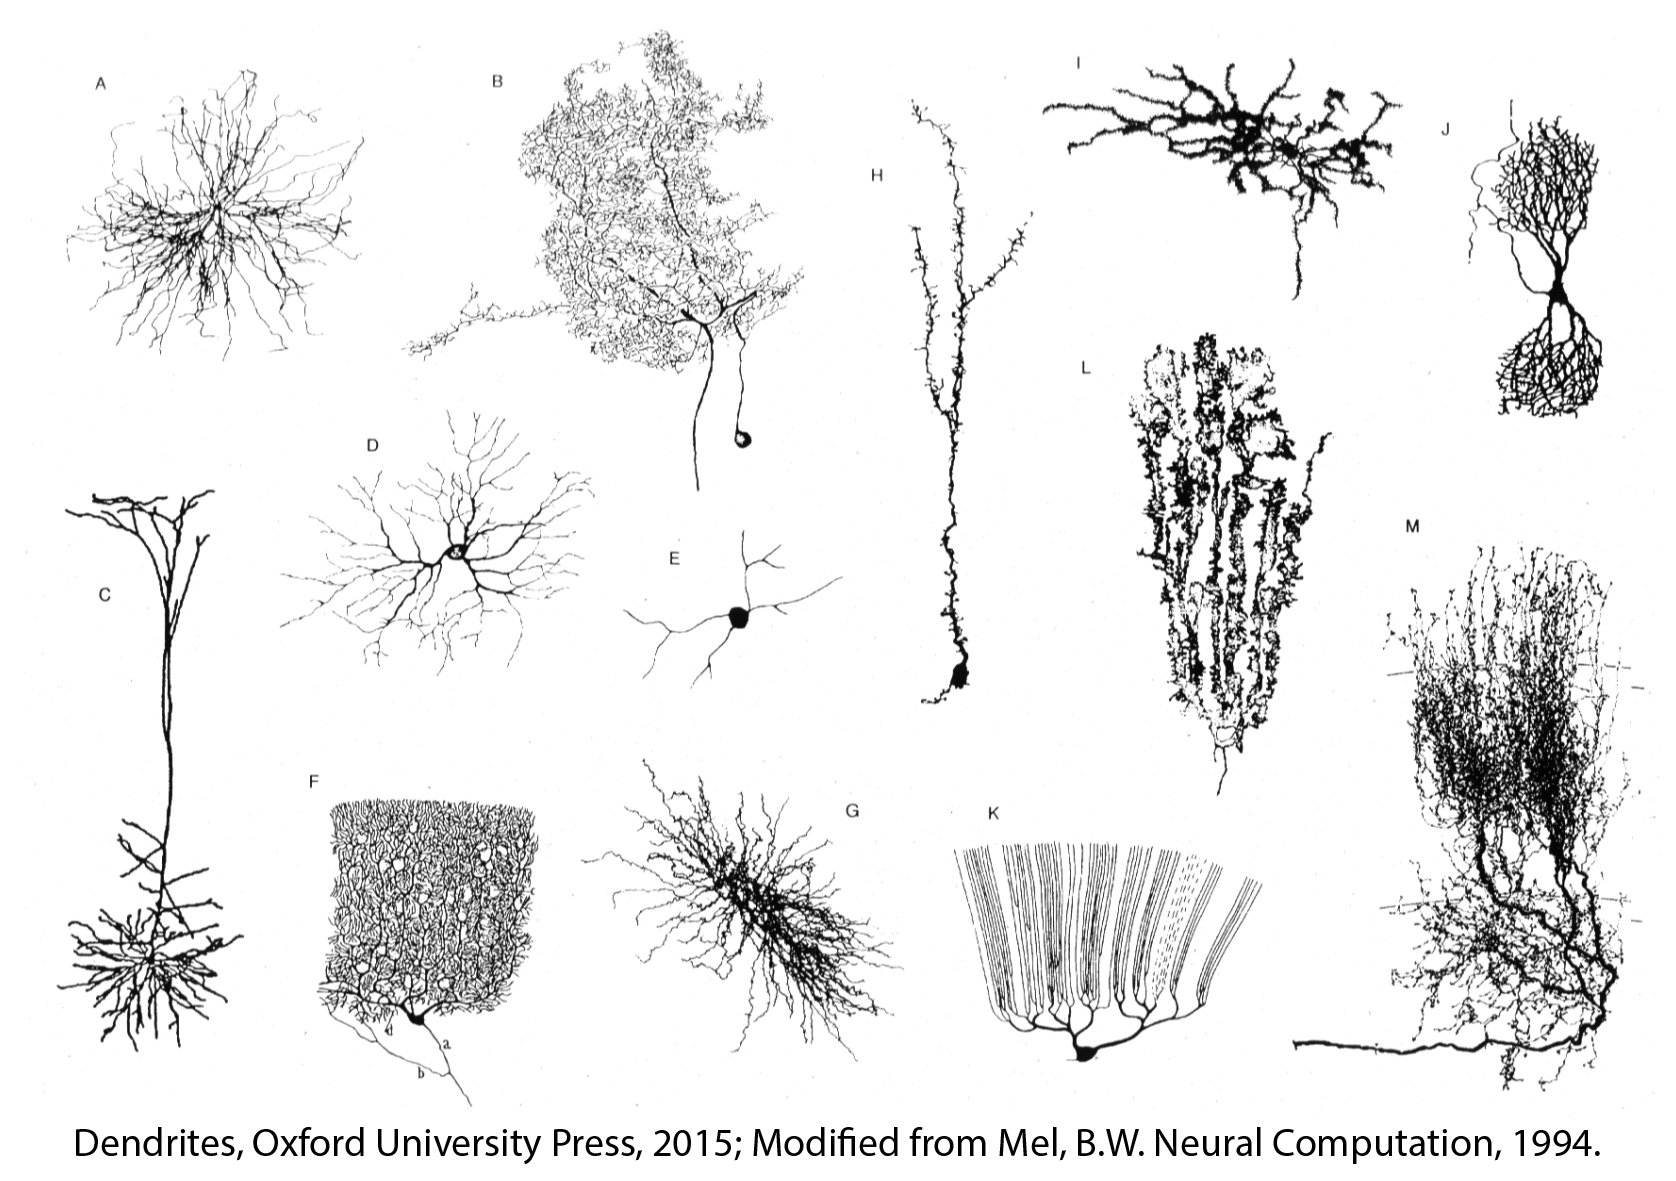
\includegraphics[width=\linewidth]{99_images/Neurons.jpg}
  \end{figure}
  \note[item]{The brain is composed of specialised cells that enable it to process information by the use of electrical impulses}
  \note[item]{As the figure shows, these cells, neurons, have specialised into many many types. They serve different functions, include different proteins and markers, and can be classified in many different ways.}
\end{frame}
\begin{frame}[t]{The brain: in numbers: neurons}
  \begin{columns}
    \begin{column}{0.5\textwidth}
      \begin{figure}[h]
        \centering
        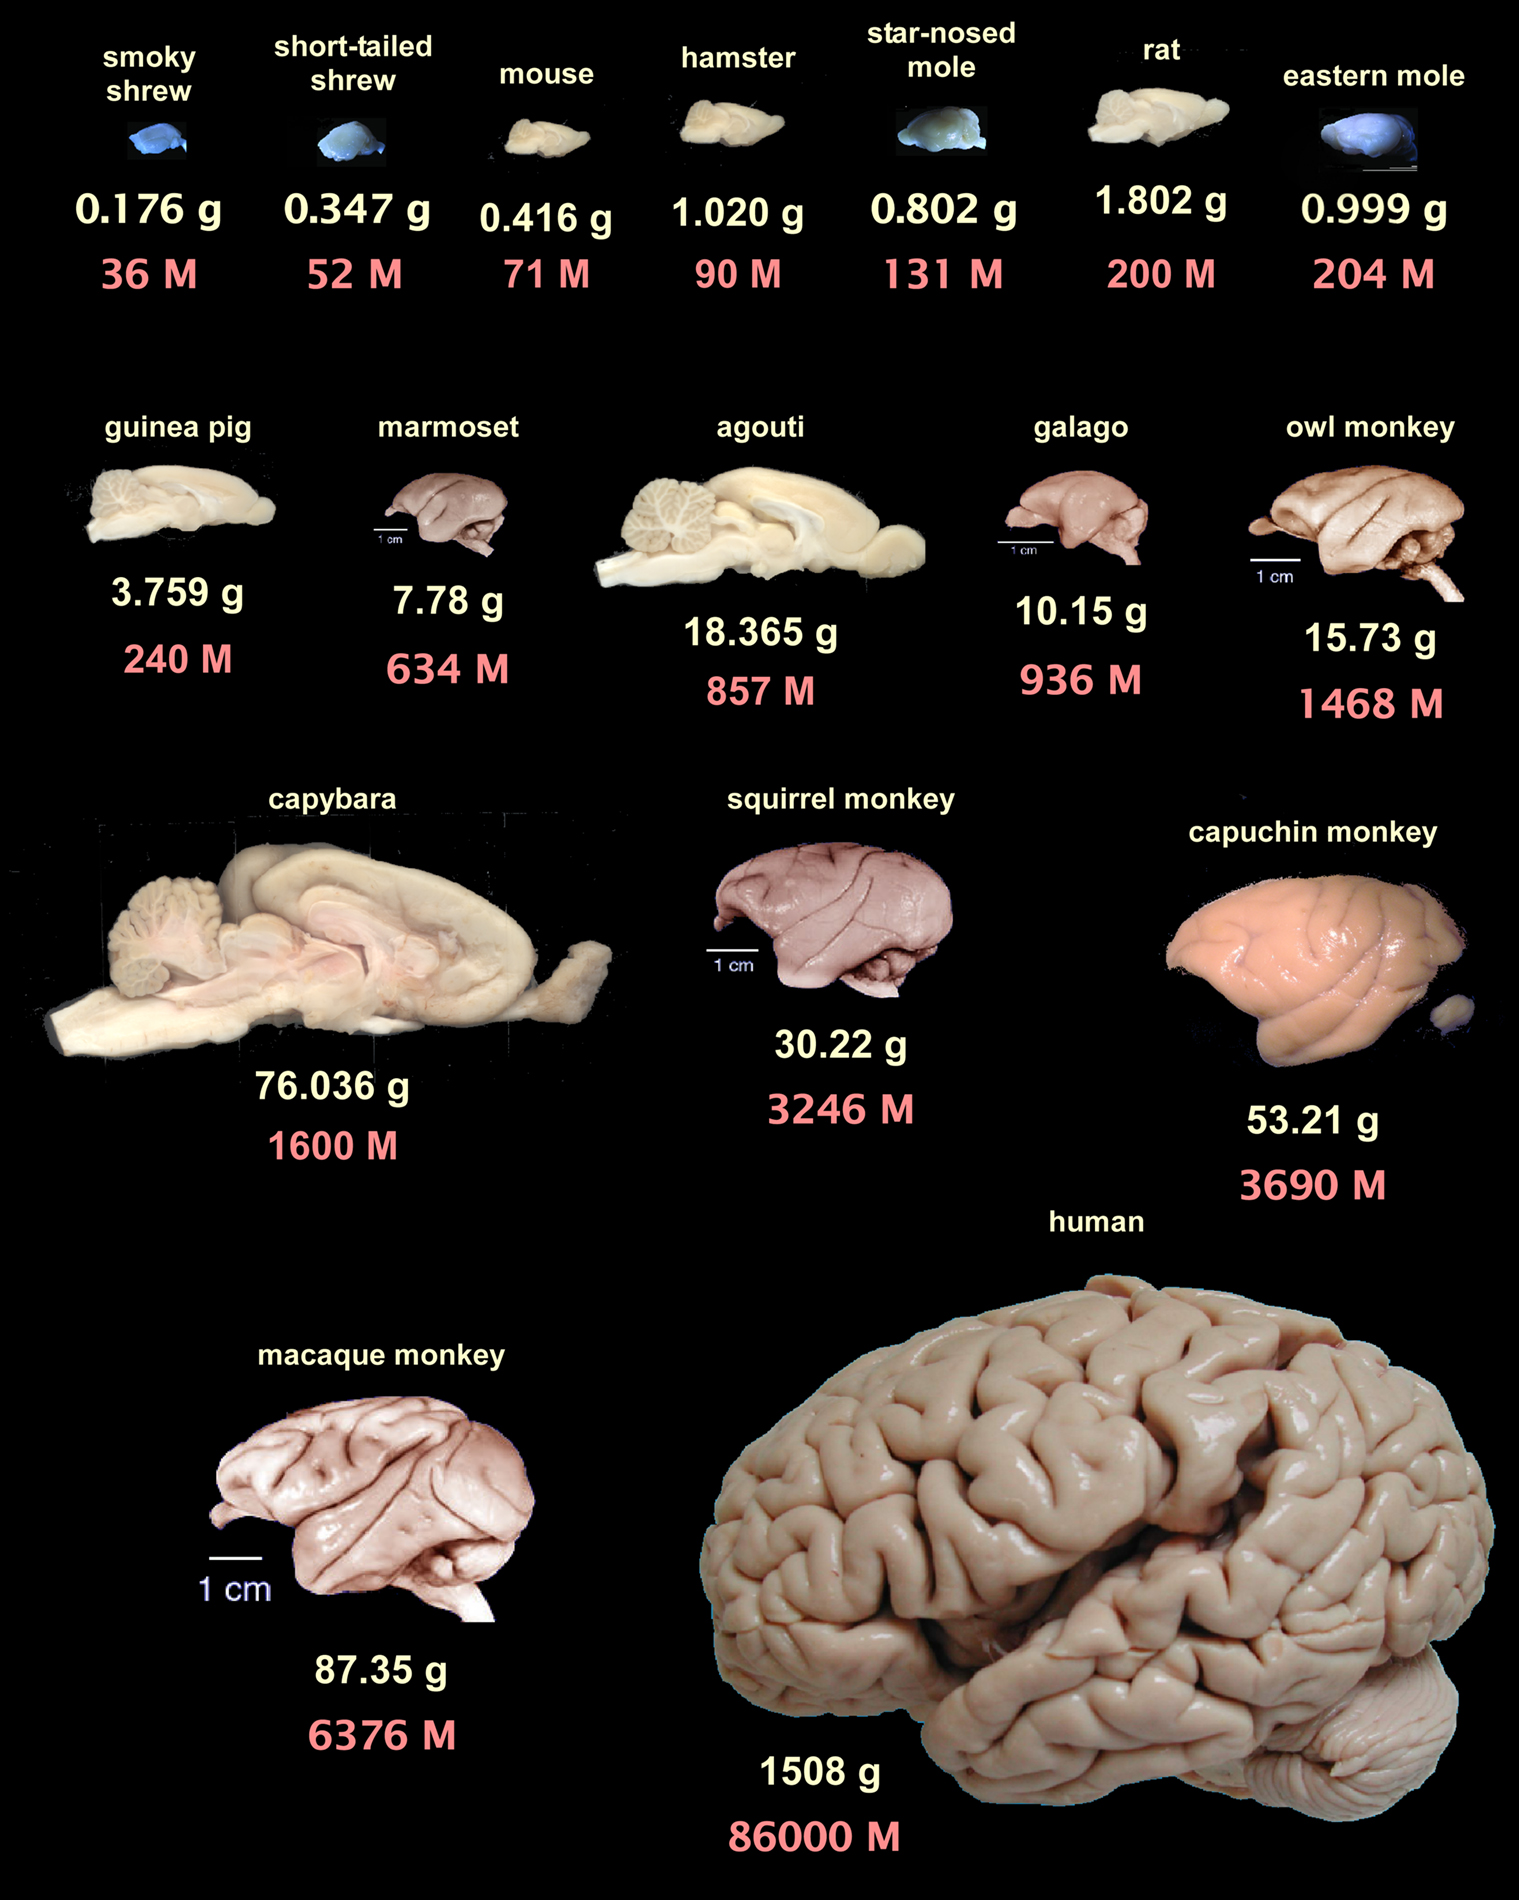
\includegraphics[width=\textwidth]{99_images/brain-sizes.jpg}
      \end{figure}
    \end{column}
    \begin{column}{0.5\textwidth}
      \begin{itemize}
        \item \alert{86000M} neurons\footnotemark{}.
        \note[item]{The most recent estimate puts the number of neurons in the human brain at 86B.}
      \end{itemize}
    \end{column}
  \end{columns}
  \vspace{0.2cm}
  \footnotetext[1]{\fullcite{Herculano-Houzel2009}}
\end{frame}
\begin{frame}[t]{The brain: in numbers: synapses}
  \begin{columns}
    \begin{column}{0.5\textwidth}
      \begin{figure}[h]
        \centering
        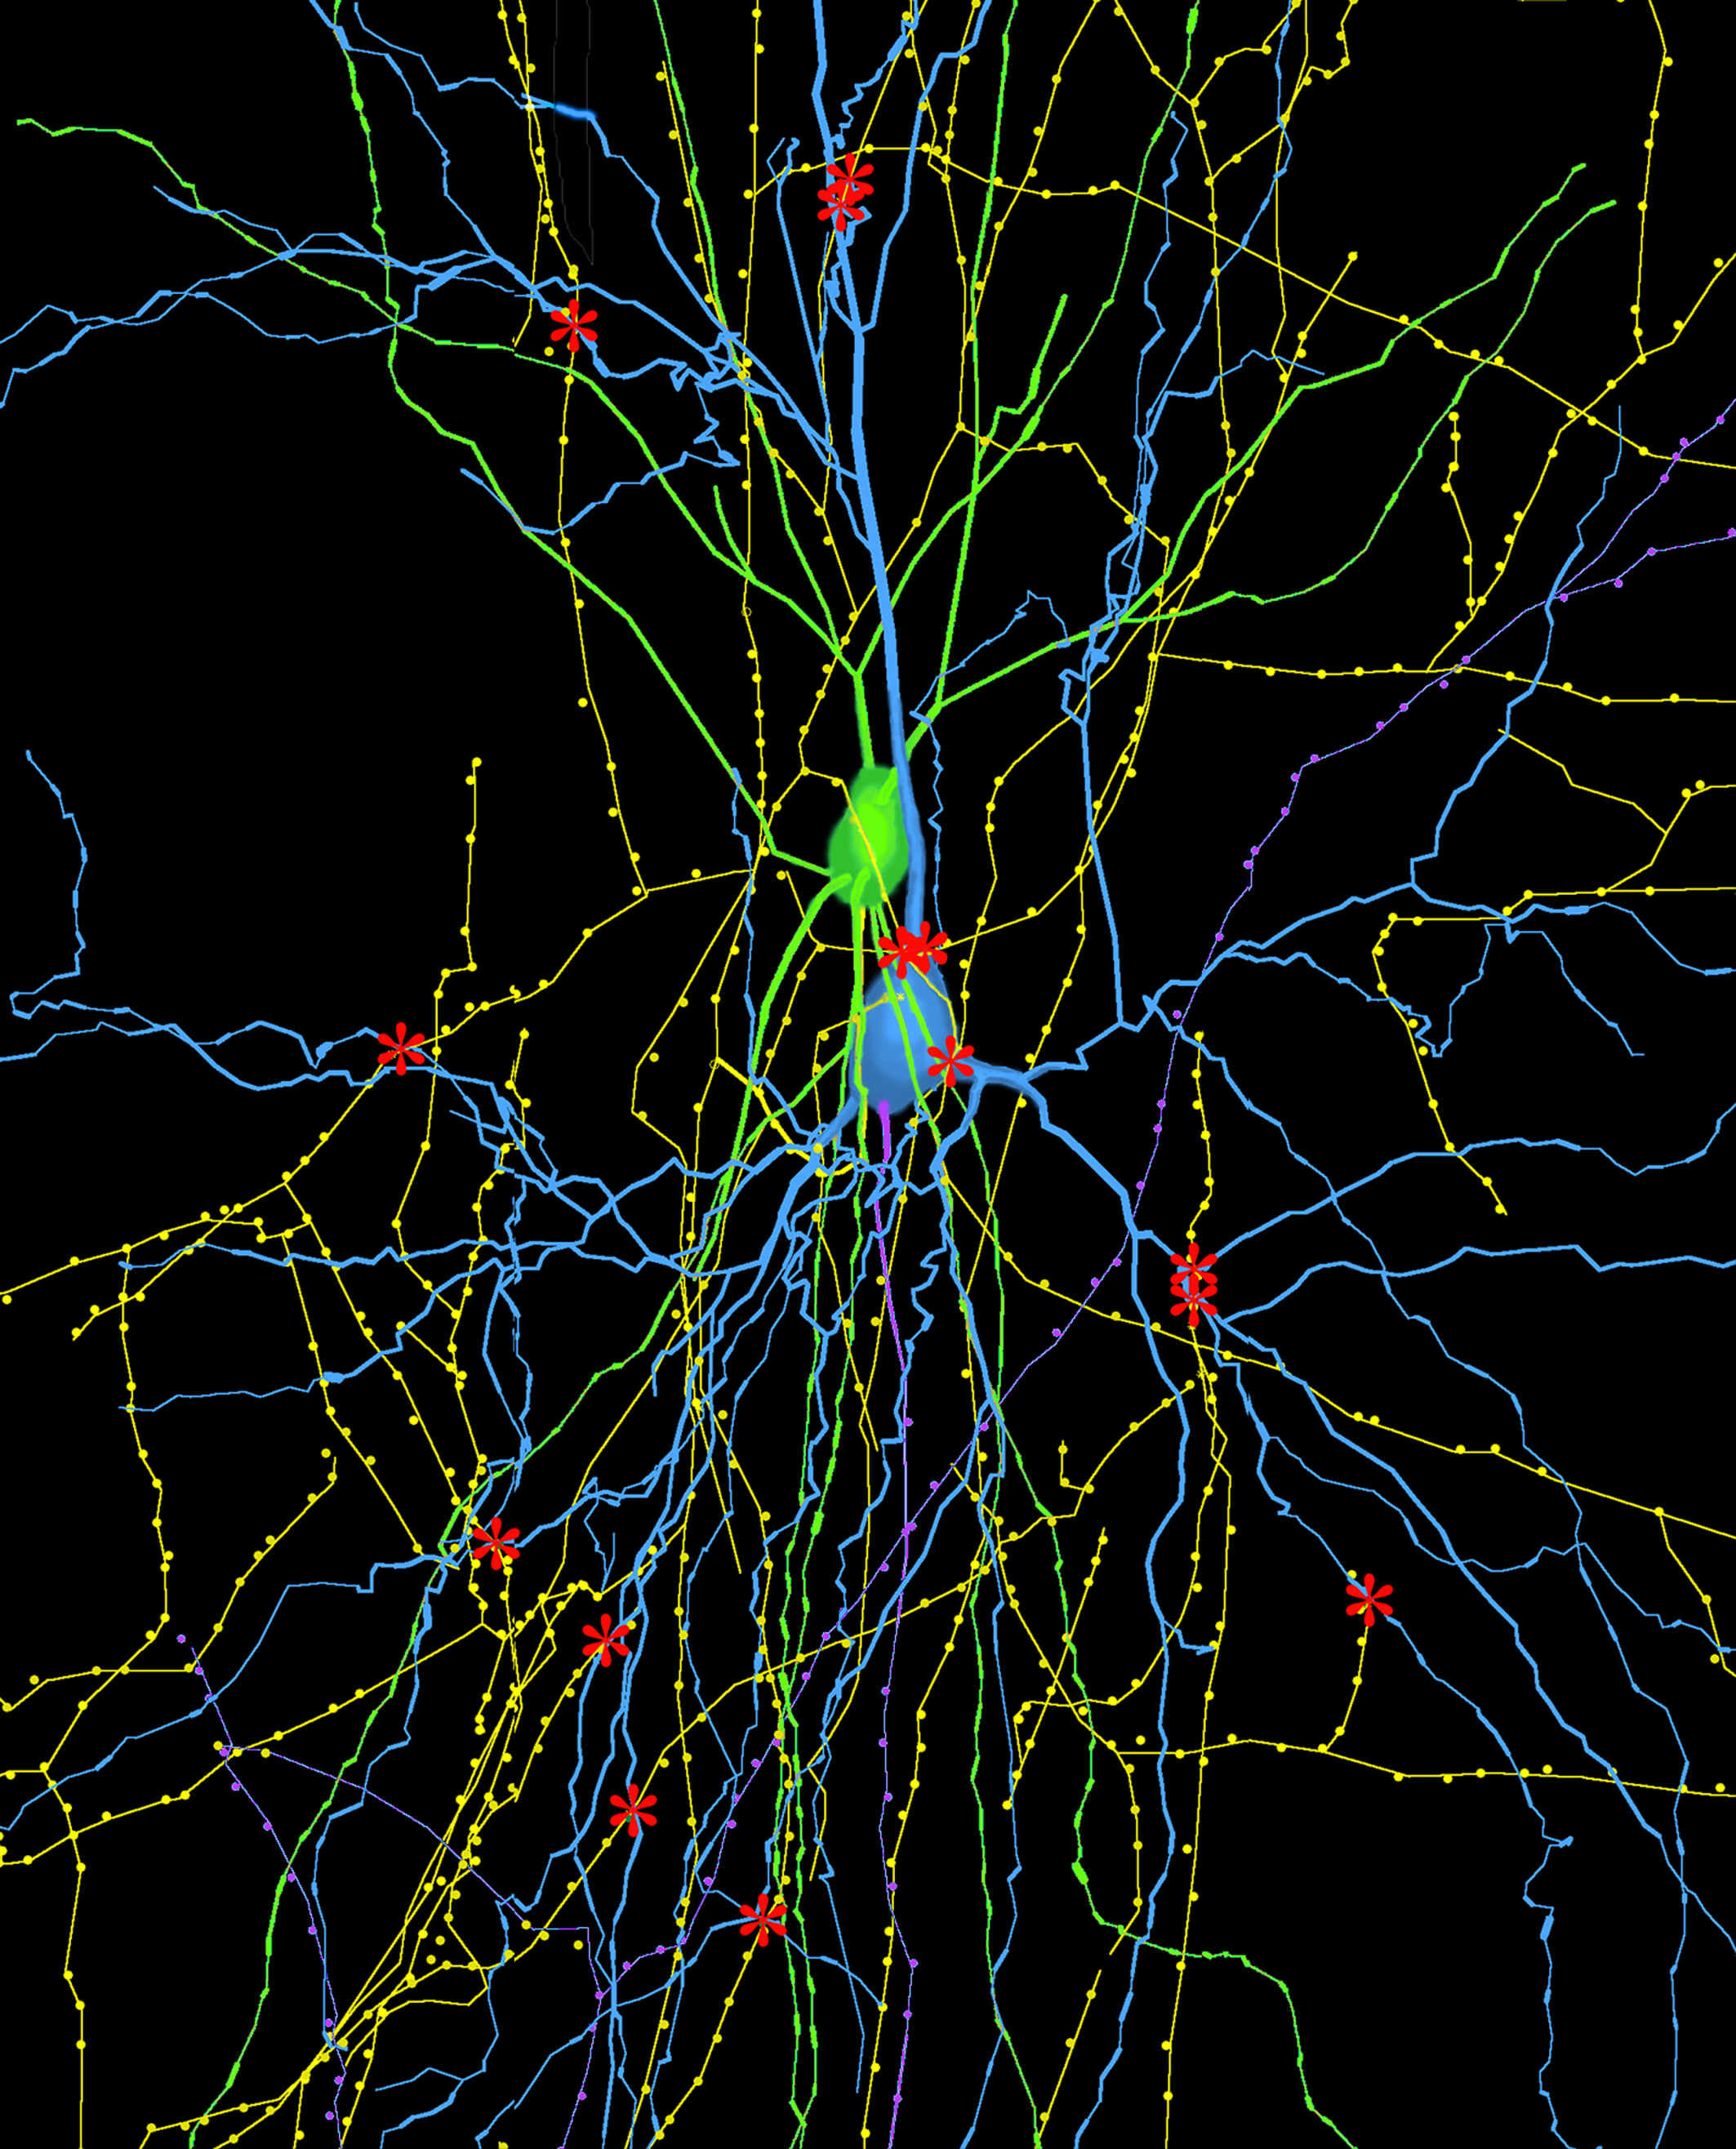
\includegraphics[width=\textwidth]{99_images/reconstruction.jpg}
      \end{figure}
    \end{column}
    \begin{column}{0.5\textwidth}
      \begin{itemize}
        \item \alert{Thousands} of connections \alert{(synapses)} between pairs\footnotemark[2].
        \note[item]{Each neuron connects with thousands of other neurons, forming a massive network.}
          \pause{}
        \item Synapses underlie \alert{learning}\footnotemark[3].
        \note[item]{This is especially important because we now know that it is in these synapses that learning occurs.}
      \end{itemize}
    \end{column}
  \end{columns}
  \vspace{0.2cm}
  \footnotetext[2]{\href{https://drexel.edu/medicine/about/departments/neurobiology-anatomy/research/gao-lab/images/}{Image from The GAO lab}}
  \footnotetext[3]{\fullcite{Hebb1949}}
\end{frame}
\begin{frame}[c]{The brain: plasticity and learning}
  \note[item]{We learn when synapses change in the brain}
  \note[item]{As an example, let's say we have a neuron that was activated by a smell.}
  \note[item]{Later, we found out that that was the smell of some food, say curry.}
  \note[item]{Because these neurons fired one after the other here, this synapse is strengthened.}
  \note[item]{When this happens repeatedly, the synapse is strengthened again and again.}
  \note[item]{Until, the faintest whiff of the smell reminds you of the food!}
  \begin{columns}
    \begin{column}{0.5\textwidth}
      \begin{figure}[h]
        \centering
        \only<1>{\def\radiusneuron{0.2cm}
\def\radiussynapse{0.02cm}
\def\lendens{0.5cm}
\def\lenax{2cm}
\begin{tikzpicture}[scale=1, transform shape]
  % Neuron 1
  \def\circlex{1.5}
  \def\circley{0}
  \draw [red] (\circlex, \circley) circle (\radiusneuron);
  \foreach \angle in {240, 270,...,360} \draw [red] ([shift=(\angle:\radiusneuron + 0.1cm )] \circlex, \circley) -- ++ (\angle:\radiusneuron+\lendens);
  \draw [red, very thick] ([shift=(120:\radiusneuron + 0.1cm )] \circlex, \circley) -- ++ (-1cm, \lenax);
  \node [red] at (\circlex, \circley - 1.5) {Smell A};
  \node [blue] at (\circlex, 3 + 1.5) {Food};

  % Neuron 2
  \def\circlex{1}
  \def\circley{3}
  \draw (\circlex, \circley) circle (\radiusneuron);
  \foreach \angle in {120, 150,...,240} \draw [blue] ([shift=(\angle:\radiusneuron + 0.1cm )] \circlex, \circley) -- ++ (\angle:\radiusneuron+\lendens);
  \draw [blue, very thick] ([shift=(0:\radiusneuron + 0.1cm )] \circlex, \circley) -- ++ (\lenax, 0);

  % Synapse
  \def\circlex{0.47}
  \def\circley{2.11}
  \draw [green, fill=green] (\circlex, \circley) circle (\radiussynapse);
\end{tikzpicture}

}
        \only<2>{\def\radiusneuron{0.2cm}
\def\radiussynapse{0.04cm}
\def\lendens{0.5cm}
\def\lenax{2cm}
\begin{tikzpicture}[scale=1, transform shape]
  % Neuron 1
  \def\circlex{1.5}
  \def\circley{0}
  \draw [red] (\circlex, \circley) circle (\radiusneuron);
  \foreach \angle in {240, 270,...,360} \draw [red] ([shift=(\angle:\radiusneuron + 0.1cm )] \circlex, \circley) -- ++ (\angle:\radiusneuron+\lendens);
  \draw [red, very thick] ([shift=(120:\radiusneuron + 0.1cm )] \circlex, \circley) -- ++ (-1cm, \lenax);
  \node [red] at (\circlex, \circley - 1.5) {Smell A};
  \node [blue] at (\circlex, 3 + 1.5) {Food};

  % Neuron 2
  \def\circlex{1}
  \def\circley{3}
  \draw (\circlex, \circley) circle (\radiusneuron);
  \foreach \angle in {120, 150,...,240} \draw [blue] ([shift=(\angle:\radiusneuron + 0.1cm )] \circlex, \circley) -- ++ (\angle:\radiusneuron+\lendens);
  \draw [blue, very thick] ([shift=(0:\radiusneuron + 0.1cm )] \circlex, \circley) -- ++ (\lenax, 0);

  % Synapse
  \def\circlex{0.47}
  \def\circley{2.11}
  \draw [green, fill=green] (\circlex, \circley) circle (\radiussynapse);
\end{tikzpicture}

}
        \only<3>{\def\radiusneuron{0.2cm}
\def\radiussynapse{0.06cm}
\def\lendens{0.5cm}
\def\lenax{2cm}
\begin{tikzpicture}[scale=1, transform shape]
  % Neuron 1
  \def\circlex{1.5}
  \def\circley{0}
  \draw [red] (\circlex, \circley) circle (\radiusneuron);
  \foreach \angle in {240, 270,...,360} \draw [red] ([shift=(\angle:\radiusneuron + 0.1cm )] \circlex, \circley) -- ++ (\angle:\radiusneuron+\lendens);
  \draw [red, very thick] ([shift=(120:\radiusneuron + 0.1cm )] \circlex, \circley) -- ++ (-1cm, \lenax);
  \node [red] at (\circlex, \circley - 1.5) {Smell A};
  \node [blue] at (\circlex, 3 + 1.5) {Food};

  % Neuron 2
  \def\circlex{1}
  \def\circley{3}
  \draw (\circlex, \circley) circle (\radiusneuron);
  \foreach \angle in {120, 150,...,240} \draw [blue] ([shift=(\angle:\radiusneuron + 0.1cm )] \circlex, \circley) -- ++ (\angle:\radiusneuron+\lendens);
  \draw [blue, very thick] ([shift=(0:\radiusneuron + 0.1cm )] \circlex, \circley) -- ++ (\lenax, 0);

  % Synapse
  \def\circlex{0.47}
  \def\circley{2.11}
  \draw [green, fill=green] (\circlex, \circley) circle (\radiussynapse);
\end{tikzpicture}

}
        \only<4>{\def\radiusneuron{0.2cm}
\def\radiussynapse{0.08cm}
\def\lendens{0.5cm}
\def\lenax{2cm}
\begin{tikzpicture}[scale=1, transform shape]
  % Neuron 1
  \def\circlex{1.5}
  \def\circley{0}
  \draw [red] (\circlex, \circley) circle (\radiusneuron);
  \foreach \angle in {240, 270,...,360} \draw [red] ([shift=(\angle:\radiusneuron + 0.1cm )] \circlex, \circley) -- ++ (\angle:\radiusneuron+\lendens);
  \draw [red, very thick] ([shift=(120:\radiusneuron + 0.1cm )] \circlex, \circley) -- ++ (-1cm, \lenax);
  \node [red] at (\circlex, \circley - 1.5) {Smell A};
  \node [blue] at (\circlex, 3 + 1.5) {Food};

  % Neuron 2
  \def\circlex{1}
  \def\circley{3}
  \draw (\circlex, \circley) circle (\radiusneuron);
  \foreach \angle in {120, 150,...,240} \draw [blue] ([shift=(\angle:\radiusneuron + 0.1cm )] \circlex, \circley) -- ++ (\angle:\radiusneuron+\lendens);
  \draw [blue, very thick] ([shift=(0:\radiusneuron + 0.1cm )] \circlex, \circley) -- ++ (\lenax, 0);

  % Synapse
  \def\circlex{0.47}
  \def\circley{2.11}
  \draw [green, fill=green] (\circlex, \circley) circle (\radiussynapse);
\end{tikzpicture}

}
        \only<5>{\def\radiusneuron{0.2cm}
\def\radiussynapse{0.10cm}
\def\lendens{0.5cm}
\def\lenax{2cm}
\begin{tikzpicture}[scale=1, transform shape]
  % Neuron 1
  \def\circlex{1.5}
  \def\circley{0}
  \draw [red] (\circlex, \circley) circle (\radiusneuron);
  \foreach \angle in {240, 270,...,360} \draw [red] ([shift=(\angle:\radiusneuron + 0.1cm )] \circlex, \circley) -- ++ (\angle:\radiusneuron+\lendens);
  \draw [red, very thick] ([shift=(120:\radiusneuron + 0.1cm )] \circlex, \circley) -- ++ (-1cm, \lenax);
  \node [red] at (\circlex, \circley - 1.5) {Smell A};
  \node [blue] at (\circlex, 3 + 1.5) {Food: curry!};

  % Neuron 2
  \def\circlex{1}
  \def\circley{3}
  \draw (\circlex, \circley) circle (\radiusneuron);
  \foreach \angle in {120, 150,...,240} \draw [blue] ([shift=(\angle:\radiusneuron + 0.1cm )] \circlex, \circley) -- ++ (\angle:\radiusneuron+\lendens);
  \draw [blue, very thick] ([shift=(0:\radiusneuron + 0.1cm )] \circlex, \circley) -- ++ (\lenax, 0);

  % Synapse
  \def\circlex{0.47}
  \def\circley{2.11}
  \draw [green, fill=green] (\circlex, \circley) circle (\radiussynapse);
\end{tikzpicture}

}
      \end{figure}
    \end{column}
    \begin{column}{0.5\textwidth}
      \begin{figure}[h]
        \centering
        \def\lenspike{0.5cm}
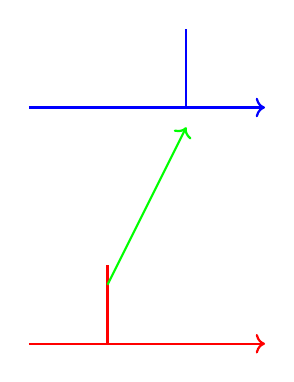
\begin{tikzpicture}[scale=1, transform shape]
  % Neuron 1
  \def\circlex{0}
  \def\circley{0}
  \draw [red, thick, ->] (\circlex, \circley) -- ++ (3cm, 0);
  \draw [red, thick] (\circlex + 1cm, \circley) -- ++ (0, \lenspike);

  \draw [green, thick, ->] (\circlex + 1cm, \circley + 0.75) -- ++ (\circlex + 1cm, 2);

  % Neuron 2
  \def\circlex{0}
  \def\circley{3}
  \draw [blue, thick, ->] (\circlex, \circley) -- ++ (3cm, 0);
  \draw [blue, thick] (\circlex + 2cm, \circley) -- ++ (0, \lenspike);
\end{tikzpicture}



      \end{figure}
    \end{column}
  \end{columns}
\end{frame}
\begin{frame}[c]{The brain: plasticity and stability?}
  \begin{itemize}
    \item Learning occurs \alert{all the time}.
      \pause{}
    \item In fact, \alert{whole synapses are formed and removed} all the time\footnotemark[4]: \textbf{structural plasticity}.
      \note[item]{Changes in whole synapses change the structure of the networks of neurons, and is referred to as structural plasticity}
      \pause{}
    \item Unregulated brain activity causes disorders: \alert{epilepsy}.
    \item So, how does the brain remain \alert{stable} despite changing all the time?
      \pause{}
      \note[item]{This led researchers to investigate stabilising processes which must work in parallel with learning}
    \item Stabilising \alert{(homeostatic)} processes\footnotemark[5]?
  \end{itemize}
  \footnotetext[4]{\fullcite{Holtmaat2005}}
  \footnotetext[5]{\fullcite{Turrigiano1999}}
\end{frame}
\begin{frame}[c]{Our research focus}
  \begin{itemize}
    \item We study \alert{homeostatic structural plasticity}.
  \end{itemize}
\end{frame}
\section{Homeostatic structural plasticity}
\begin{frame}[c]{Studying homeostatic structural plasticity: biologists}
  \note[item]{The protocol is pretty standard. Here, for a study in the visual cortex, the retinal field of a rat or a mouse is mapped.}
  \begin{columns}
    \begin{column}{0.5\textwidth}
      \centering
      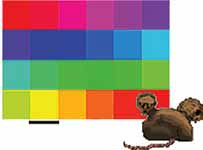
\includegraphics[width=0.8\textwidth]{99_images/keck-1-1a}%chktex 8
    \end{column}
    \begin{column}{0.5\textwidth}
      \centering
      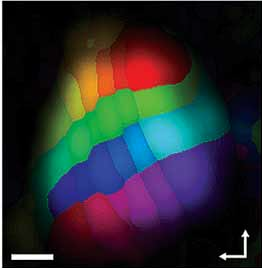
\includegraphics[width=0.8\textwidth]{99_images/keck-1-1c}%chktex 8
    \end{column}
  \end{columns}
  \footnotetext[1]{\fullcite{Keck2008}}
\end{frame}

\begin{frame}[c]{after injury \ldots}
  \note[item]{Then, a part of the retina is lesioned. This cuts off inputs to a part of the visual cortex, as shown in the first figure. This forms the Lesion Projection Zone (LPZ). By repeated imaging of the region over months, the reorganisation of the network is tracked.}
  \note[item]{Other lesion studies use similar methods: digit removal, whisker trimming, and so on---anything that cuts off projecting activity on to a set of neurons.}
    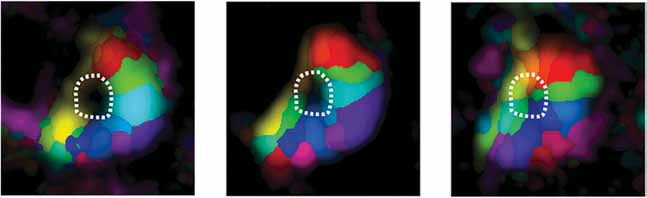
\includegraphics[width=\textwidth]{99_images/keck-1-2c}%chktex 8
    \footnotetext[1]{\fullcite{Keck2008}}
\end{frame}
\begin{frame}[c]{Our investigations: computational modelling}
  \begin{itemize}
    \item We make \alert{models of small parts of the brain} on computers.
      \note[item]{Really small parts: 10000 neurons only}
    \item We try to \alert{replicate} what biologists observe in their laboratories.
      \pause{}
    \item Modelling gives us \alert{flexibility}:
      \begin{itemize}
        \item we can change whatever we want, record whatever we want.
        \item analyse data, test different hypotheses.
      \end{itemize}
      \pause{}
    \item We then \alert{send our ideas back to biologists} for validation.
  \end{itemize}
\end{frame}
\begin{frame}[c]{Our model: replicates biological observations}
  \begin{figure}
      \centering
      \resizebox{\textwidth}{!}{% GNUPLOT: LaTeX picture with Postscript
\begingroup
  \makeatletter
  \providecommand\color[2][]{%
    \GenericError{(gnuplot) \space\space\space\@spaces}{%
      Package color not loaded in conjunction with
      terminal option `colourtext'%
    }{See the gnuplot documentation for explanation.%
    }{Either use 'blacktext' in gnuplot or load the package
      color.sty in LaTeX.}%
    \renewcommand\color[2][]{}%
  }%
  \providecommand\includegraphics[2][]{%
    \GenericError{(gnuplot) \space\space\space\@spaces}{%
      Package graphicx or graphics not loaded%
    }{See the gnuplot documentation for explanation.%
    }{The gnuplot epslatex terminal needs graphicx.sty or graphics.sty.}%
    \renewcommand\includegraphics[2][]{}%
  }%
  \providecommand\rotatebox[2]{#2}%
  \@ifundefined{ifGPcolor}{%
    \newif\ifGPcolor
    \GPcolortrue
  }{}%
  \@ifundefined{ifGPblacktext}{%
    \newif\ifGPblacktext
    \GPblacktexttrue
  }{}%
  % define a \g@addto@macro without @ in the name:
  \let\gplgaddtomacro\g@addto@macro
  % define empty templates for all commands taking text:
  \gdef\gplbacktext{}%
  \gdef\gplfronttext{}%
  \makeatother
  \ifGPblacktext
    % no textcolor at all
    \def\colorrgb#1{}%
    \def\colorgray#1{}%
  \else
    % gray or color?
    \ifGPcolor
      \def\colorrgb#1{\color[rgb]{#1}}%
      \def\colorgray#1{\color[gray]{#1}}%
      \expandafter\def\csname LTw\endcsname{\color{white}}%
      \expandafter\def\csname LTb\endcsname{\color{black}}%
      \expandafter\def\csname LTa\endcsname{\color{black}}%
      \expandafter\def\csname LT0\endcsname{\color[rgb]{1,0,0}}%
      \expandafter\def\csname LT1\endcsname{\color[rgb]{0,1,0}}%
      \expandafter\def\csname LT2\endcsname{\color[rgb]{0,0,1}}%
      \expandafter\def\csname LT3\endcsname{\color[rgb]{1,0,1}}%
      \expandafter\def\csname LT4\endcsname{\color[rgb]{0,1,1}}%
      \expandafter\def\csname LT5\endcsname{\color[rgb]{1,1,0}}%
      \expandafter\def\csname LT6\endcsname{\color[rgb]{0,0,0}}%
      \expandafter\def\csname LT7\endcsname{\color[rgb]{1,0.3,0}}%
      \expandafter\def\csname LT8\endcsname{\color[rgb]{0.5,0.5,0.5}}%
    \else
      % gray
      \def\colorrgb#1{\color{black}}%
      \def\colorgray#1{\color[gray]{#1}}%
      \expandafter\def\csname LTw\endcsname{\color{white}}%
      \expandafter\def\csname LTb\endcsname{\color{black}}%
      \expandafter\def\csname LTa\endcsname{\color{black}}%
      \expandafter\def\csname LT0\endcsname{\color{black}}%
      \expandafter\def\csname LT1\endcsname{\color{black}}%
      \expandafter\def\csname LT2\endcsname{\color{black}}%
      \expandafter\def\csname LT3\endcsname{\color{black}}%
      \expandafter\def\csname LT4\endcsname{\color{black}}%
      \expandafter\def\csname LT5\endcsname{\color{black}}%
      \expandafter\def\csname LT6\endcsname{\color{black}}%
      \expandafter\def\csname LT7\endcsname{\color{black}}%
      \expandafter\def\csname LT8\endcsname{\color{black}}%
    \fi
  \fi
    \setlength{\unitlength}{0.0500bp}%
    \ifx\gptboxheight\undefined%
      \newlength{\gptboxheight}%
      \newlength{\gptboxwidth}%
      \newsavebox{\gptboxtext}%
    \fi%
    \setlength{\fboxrule}{0.5pt}%
    \setlength{\fboxsep}{1pt}%
\begin{picture}(7936.00,2550.00)%
    \gplgaddtomacro\gplbacktext{%
    }%
    \gplgaddtomacro\gplfronttext{%
    }%
    \gplgaddtomacro\gplbacktext{%
    }%
    \gplgaddtomacro\gplfronttext{%
    }%
    \gplgaddtomacro\gplbacktext{%
    }%
    \gplgaddtomacro\gplfronttext{%
    }%
    \gplgaddtomacro\gplbacktext{%
    }%
    \gplgaddtomacro\gplfronttext{%
      \csname LTb\endcsname%
      \put(7554,51){\makebox(0,0)[l]{\strut{}$1$}}%
      \put(7554,2285){\makebox(0,0)[l]{\strut{}$5$}}%
      \put(7752,1168){\rotatebox{-270}{\makebox(0,0){\strut{}Firing rate (Hz)}}}%
    }%
    \gplbacktext
    \put(0,0){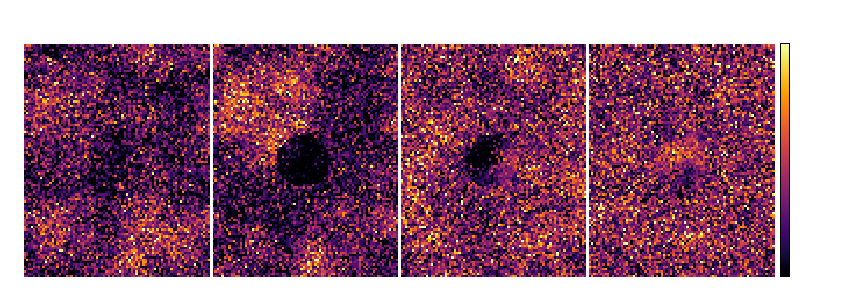
\includegraphics[interpolate=false]{99_images/201811221433-firing-rate-snapshots-E}}%
    \gplfronttext
  \end{picture}%
\endgroup
}%
      \caption{Our model: 1000 neurons. Simulation duration: 7 days on the cluster with 128 CPU nodes.}
  \end{figure}
\end{frame}
\begin{frame}[c]{It suggests:}

\end{frame}
\end{document}
